\section{The CnC Programming Model}

The Concurrent Collections Programming Model (CnC), developed by Intel, is one such data-centric programming model.  Its deterministic semantics allow a task-based runtime to programmatically exploit parallelism.  In addition, it allows for a secondary file, called a tuning spec, to provide additional hints to improve performance.

\begin{figure}[!htb]
  \centering
  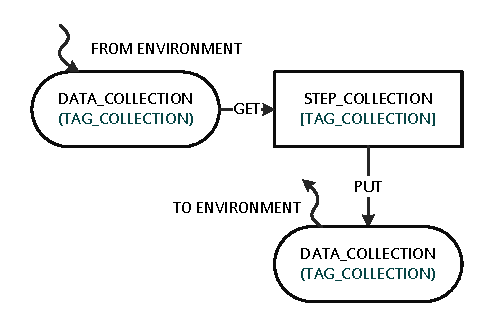
\includegraphics[width=0.5\textwidth]{drawings/CnCExample.pdf}
  \caption{CnC Semanticcs Graph}
  \label{fig:cnc_graph}
\end{figure}

The CnC model can be thought of as a producer-consumer paradigm where data is produced and consumed by tasks, or Steps in CnC terminology.  The produced and consumed data is declared explicitly in an input file, known as a CnC graph file.  The steps themselves are also entities that can be produced.  When a step produces another tasks, this is known as control dependencies and is also declared in the CnC graph file.  Figure \ref{fig:cnc_graph} shows a visual representation of a CnC graph file.  The figure shows the steps (rectangles), the data (ovals), and the dependencies between them.  The title of a step is often a verb, describing the work being done within the step.  The title of a data collection is often a noun, describing the data within the collection.  The control dependencies are not shown.  A text based version of the same data, including the control dependencies, is provided to CnC when designing a CnC application, an example of which is given in section 5.

By declaring all dependencies between steps and data the specifics regarding how the algorithm is executed is  abstracted out of the implementation.  As an example, it is clear what data is needed by a given step.  If that data has not been produced yet, the step will not be scheduled.  This allows the runtime to optimally decide when and where to schedule computation. For some more complicated semantic, additional hints can be provided to the runtime through a separate file called a tuning specification.  This is also useful for running the same program on different architectures, as no rewrites of the application are necessary to switch platforms just the tuning specification. 

\subsection{Language Specifics}
The CnC model is built on three key constructs; step collections, data collections, and control collections ~\cite{budimlicconcurrent}. A step collection defines computation, an instance of which consumes and produces data.  The consumed and produced data, or data items, belong to data collections.  Data items within a data collection are indexed using item tags.  Tags can be thought of as tuples and can be anything that can uniquely identify one given instance of the data in the data's collection.  Finally the control collection describes the prescription, or creation, of step instances.  The relationship between these collections as well as the collections themselves are defined in the CnC graph file.

Developing a CnC application then begins with designing the CnC graph file. An algorithm is broken down into computation steps, instances of which correspond to different input arguments. These steps along with the data collections become nodes in a graph. Each step can optionally consume data, produce data, and prescribe additional computation. These relationships, producer, consumer, and control, define the edges in the graph and will dynamically be satisfied as the program executes.

The next and final required step in producing a CnC application is to implement the step logic. The flow within a single CnC step is as follows: consume, compute and produce. This ordering is required as there is no guarantee the data a step needs will be ready when the step begins executing. This is due to steps being preemptively scheduled when they are prescribed.  Most of the time the data will be ready when a steps begins execution, occasionally and often due to implementation error a step’s data may never be available.  Internally if the data is not ready when a CnC step begins execution it will halt execution and try again later. To improve performance, hints can be provided through the tuning specification to increase the likelihood that steps are schedule for execution when their required input data is ready.

\subsection{CnC Example}

\begin{figure}[!htb]
  \centering
  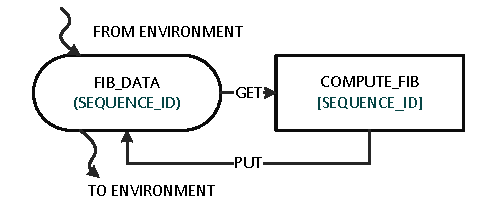
\includegraphics[width=0.5\textwidth]{drawings/FibExample.pdf}
  \caption{CnC Graph: Fibonacci}
  \label{fig:fib_graph}
\end{figure}

% apparently putting this here makes it show up on the top of page 3, where I want it
\begin{figure*}[!htb]
  \centering
  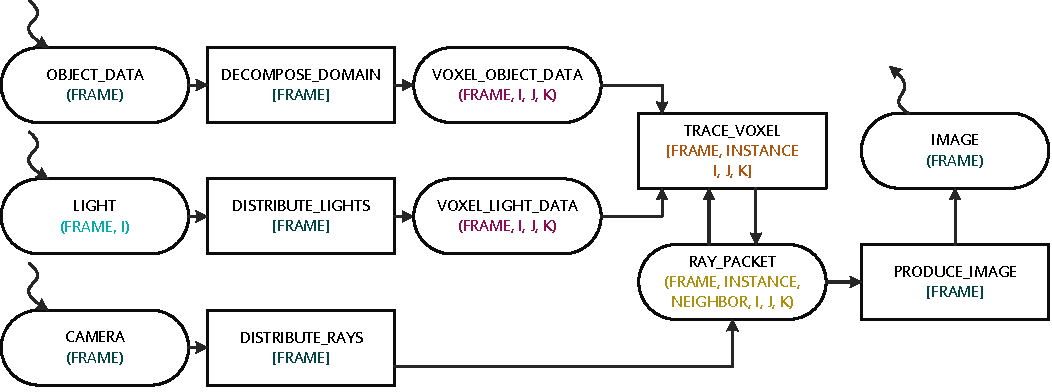
\includegraphics[width=\textwidth]{drawings/CnC.pdf}
  \caption{CnC Graph}
  \label{fig:cnc}
\end{figure*}

As an example, we may consider a simple recursive implementation of the Fibonacci sequence, see figure \ref{fig:fib_graph}.  This application consists of one step, COMPUTE\_FIB, which takes the previous two computed values as input and produces the next value in the sequence.  One data collection, FIB\_DATA exists for the application.  Data within the collection is indexed by a tag consisting of the values sequence number. Tags 1-5, then point to the values 1, 1, 2, 3, 5, respectively.  The first two values of the data collection are produced by the environment, the rest of the values in the collection are produced as needed by COMPUTE\_FIB.  A tag exists for COMPUTE\_FIB as well.  We can index this collection by the integer sequence a particular instance will produce.  For example the step instance at tag 3 will consume the data at tag 1 and 2, and produce data at tag 3.  Specifically it will consume 1, 1 and produce 2.  The number of steps executed in this example is produced by the environment.

%%% Local Variables: 
%%% mode: latex
%%% TeX-master: "main"
%%% End: 
